\chapter{Experiments and Discussion}



In this chapter we collect the plots of the \nameref{c:experiments} and \nameref{c:discussion} chapters that would have cluttered the chapters to much while not adding much information.

\section{Plots for Running on the CPU or GPU}
	\label{app:plotsCpuGpu}

	Plot overview:
	\begin{itemize}
		\item Double pendulum experiment on \ac{cpu}:~\autoref{fig:cpuVsGpuCpu}
		\item Double pendulum experiment on \ac{gpu}:~\autoref{fig:cpuVsGpuCpu}
	\end{itemize}

	\begin{figure}
		\centering
		\includegraphics[width=\linewidth]{figures/results/cpu-vs-gpu/acrobot-gpu/rollout-observations-N0.png}
		\caption[Rollout of the double pendulum experiment that ran on the CPU]{Rollout of the double pendulum experiment that ran on the CPU.}
		\label{fig:cpuVsGpuCpu}
	\end{figure}
	\begin{figure}
		\centering
		\includegraphics[width=\linewidth]{figures/results/cpu-vs-gpu/acrobot-gpu/rollout-observations-N0.png}
		\caption[Rollout of the double pendulum experiment that ran on the GPU]{Rollout of the double pendulum experiment that ran on the GPU.}
		\label{fig:cpuVsGpuGpu}
	\end{figure}
% end

\section{Plots for Single- and Multi-Sequence Learning}
	\label{app:plotsSingleMulti}

	Plot overview:
	\begin{itemize}
		\item Damped pendulum experiment on a single observation sequence:~\autoref{fig:plotsSingleSequence}
		\item Damped pendulum experiment on a multiple (two) observation sequence:~\autoref{fig:plotsMultiSequence}
	\end{itemize}

	\begin{figure}
		\centering
		\includegraphics[width=\linewidth]{figures/results/single-vs-multi-sequence/pendulum-damped-single/rollout-observations-N0.png}
		\caption[Rollout of the damped pendulum experiment learning on a single observation sequence]{Rollout of the damped pendulum experiment learning on a single observation sequence.}
		\label{fig:plotsSingleSequence}
	\end{figure}
	\begin{figure}
		\centering
		\begin{subfigure}{\linewidth}
			\includegraphics[width=\linewidth]{figures/results/single-vs-multi-sequence/pendulum-damped-multi/rollout-observations-N0.png}
		\end{subfigure} \\
		\begin{subfigure}{\linewidth}
			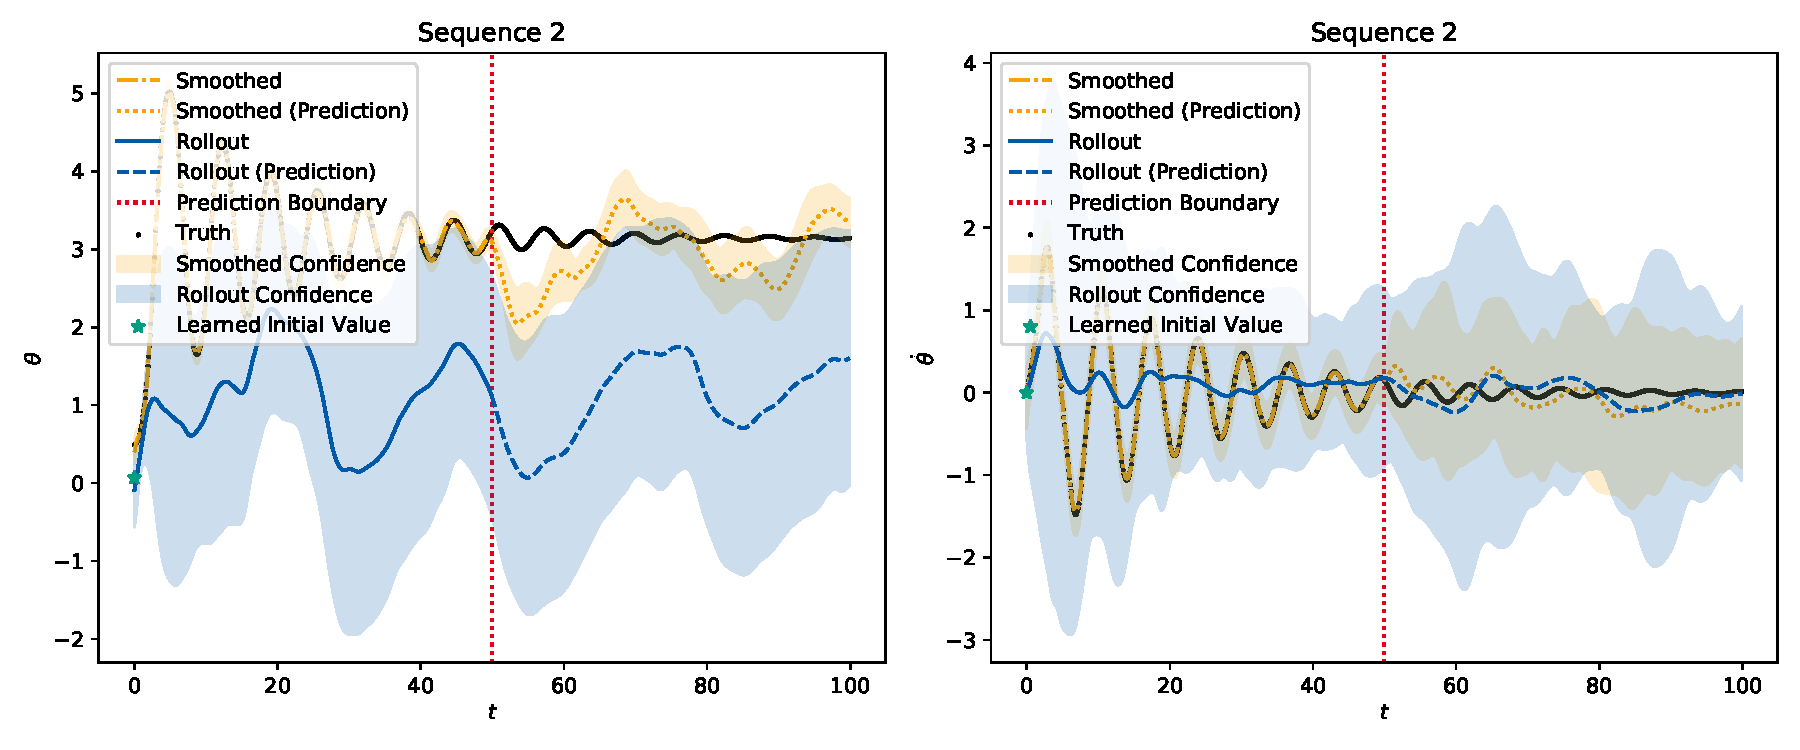
\includegraphics[width=\linewidth]{figures/results/single-vs-multi-sequence/pendulum-damped-multi/rollout-observations-N1.png}
		\end{subfigure}
		\caption[Rollout of the damped pendulum experiment learning on two observation sequences]{Rollout of the damped pendulum experiment learning on multiple (two) observation sequences. The top row is the first observation sequence, the bottom row is the second observation sequence.}
		\label{fig:plotsMultiSequence}
	\end{figure}
% end

\section{Remaining Plots}
	\label{app:remainingPlots}

	\subsection{Pendulum}
		Plot overview:
		\begin{itemize}
			\item Pendulum, 2-dimensional latent:~\autoref{fig:pendulumRolloutL02}
			\item Pendulum, 14-dimensional latent:~\autoref{fig:pendulumRolloutL14}
		\end{itemize}

		\begin{figure}
			\centering
			\includegraphics[width=\linewidth]{figures/results/pendulum/run-latent-dim-02/rollout-observations-N0.png}
			\caption[Rollout of the pendulum experiment for 2 latent dimensions]{The rollout plot in the observation space of the pendulum environment for \(k = 2\). The left plot shows the displacement and the right plot the angular velocity. The black dots represent the true data of which the model used everything until the red prediction boundary to train on. The blue line is the rollout, starting from the learned initial value (marked with a green star). The orange dash-dotted line is the smoothed data. The dotted orange line then is the rollout starting from the last smoothed state, forming the "smoothed prediction". The shaded regions show the confidence, \ie two times the standard deviation.}
			\label{fig:pendulumRolloutL02}
		\end{figure}

		\begin{figure}
			\centering
			\includegraphics[width=\linewidth]{figures/results/pendulum/run-latent-dim-14/rollout-observations-N0.png}
			\caption[Rollout of the pendulum experiment for 14 latent dimensions]{The rollout plot in the observation space of the pendulum environment for \(k = 14\). The left plot shows the displacement and the right plot the angular velocity. The black dots represent the true data of which the model used everything until the red prediction boundary to train on. The blue line is the rollout, starting from the learned initial value (marked with a green star). The orange dash-dotted line is the smoothed data. The dotted orange line then is the rollout starting from the last smoothed state, forming the "smoothed prediction". The shaded regions show the confidence, \ie two times the standard deviation.}
			\label{fig:pendulumRolloutL14}
		\end{figure}
	% end

	\subsection{Damped Pendulum}
		Plot overview:
		\begin{itemize}
			\item Damped pendulum, 2-dimensional latent:~\autoref{fig:pendulumDampedRolloutL02}
			\item Damped pendulum, 30-dimensional latent:~\autoref{fig:pendulumDampedRolloutL30}
		\end{itemize}

		\begin{figure}
			\centering
			\includegraphics[width=\linewidth]{figures/results/pendulum-damped/run-latent-dim-02/rollout-observations-N0.png}
			\caption[Rollout of the damped pendulum experiment for 2 latent dimensions]{The rollout plot in the observation space of the damped pendulum environment for \(k = 2\). The left plot shows the displacement and the right plot the angular velocity. The black dots represent the true data of which the model used everything until the red prediction boundary to train on. The blue line is the rollout, starting from the learned initial value (marked with a green star). The orange dash-dotted line is the smoothed data. The dotted orange line then is the rollout starting from the last smoothed state, forming the "smoothed prediction". The shaded regions show the confidence, \ie two times the standard deviation.}
			\label{fig:pendulumDampedRolloutL02}
		\end{figure}

		\begin{figure}
			\centering
			\includegraphics[width=\linewidth]{figures/results/pendulum-damped/run-latent-dim-30/rollout-observations-N0.png}
			\caption[Rollout of the damped pendulum experiment for 30 latent dimensions]{The rollout plot in the observation space of the damped pendulum environment for \(k = 30\). The left plot shows the displacement and the right plot the angular velocity. The black dots represent the true data of which the model used everything until the red prediction boundary to train on. The blue line is the rollout, starting from the learned initial value (marked with a green star). The orange dash-dotted line is the smoothed data. The dotted orange line then is the rollout starting from the last smoothed state, forming the "smoothed prediction". The shaded regions show the confidence, \ie two times the standard deviation.}
			\label{fig:pendulumDampedRolloutL30}
		\end{figure}
	% end

	\subsection{Gym Pendulum}
		Plot overview:
		\begin{itemize}
			\item Gym pendulum, 2-dimensional latent:~\autoref{fig:gymPendulumRolloutL02}
			\item Gym pendulum, 7-dimensional latent:~\autoref{fig:gymPendulumRolloutL7}
		\end{itemize}

		\begin{figure}
			\centering
			\includegraphics[width=\linewidth]{figures/results/pendulum-gym/run-latent-dim-02/rollout-observations-N0.png}
			\caption[Rollout of the Gym pendulum experiment for 2 latent dimensions]{The rollout plot in the observation space of the Gym pendulum environment for \(k = 2\). The left plot shows the displacement and the right plot the angular velocity. The black dots represent the true data of which the model used everything until the red prediction boundary to train on. The blue line is the rollout, starting from the learned initial value (marked with a green star). The orange dash-dotted line is the smoothed data. The dotted orange line then is the rollout starting from the last smoothed state, forming the "smoothed prediction". The shaded regions show the confidence, \ie two times the standard deviation.}
			\label{fig:gymPendulumRolloutL02}
		\end{figure}

		\begin{figure}
			\centering
			\includegraphics[width=\linewidth]{figures/results/pendulum-gym/run-latent-dim-07/rollout-observations-N0.png}
			\caption[Rollout of the Gym pendulum experiment for 7 latent dimensions]{The rollout plot in the observation space of the pendulum environment for \(k = 7\). The left plot shows the displacement and the right plot the angular velocity. The black dots represent the true data of which the model used everything until the red prediction boundary to train on. The blue line is the rollout, starting from the learned initial value (marked with a green star). The orange dash-dotted line is the smoothed data. The dotted orange line then is the rollout starting from the last smoothed state, forming the "smoothed prediction". The shaded regions show the confidence, \ie two times the standard deviation.}
			\label{fig:gymPendulumRolloutL7}
		\end{figure}
	% end

	\subsection{Gym Cartpole}
		Plot overview:
		\begin{itemize}
			\item Cartpole, 2-dimensional latent rollout without confidence:~\autoref{fig:cartpoleRolloutL02}, with confidence:~\autoref{fig:cartpoleRolloutL02Appendix}
			\item Cartpole, 10-dimensional latent, rollout without confidence:~\autoref{fig:cartpoleRolloutL10Appendix}
			\item Cartpole, 14-dimensional latent rollout with confidence:~\autoref{fig:cartpoleRolloutL16}, without confidence:~\autoref{fig:cartpoleRolloutL16Appendix}
		\end{itemize}

		\begin{figure}
			\centering
			\includegraphics[width=\linewidth]{figures/results/cartpole-gym/run-latent-dim-02/without-confidence/rollout-observations-N0.png}
			\caption[Rollout of the cartpole experiment for 2 latent dimensions without confidence]{The rollout plot in the observation space of the cartpole environment for \(k = 2\). The top plot is the cart position (left) and velocity (right), the row the pole displacement (left) and angular velocity (right). The black dots represent the true data of which the model used everything until the red prediction boundary to train on. The blue line is the rollout, starting from the learned initial value (marked with a green star). The orange dash-dotted line is the smoothed data. The dotted orange line then is the rollout starting from the last smoothed state, forming the "smoothed prediction". Note that we have removed the confidence on this plot as it is really low, resulting in high variances. See~\autoref{fig:cartpoleRolloutL02Appendix} in~\autoref{app:remainingPlots} for the plot with confidence.}
			\label{fig:cartpoleRolloutL02}
		\end{figure}
		\begin{figure}
			\centering
			\includegraphics[width=\linewidth]{figures/results/cartpole-gym/run-latent-dim-02/rollout-observations-N0.png}
			\caption[Rollout of the cartpole experiment for 2 latent dimensions with confidence]{This plot shows the same data as in~\autoref{fig:cartpoleRolloutL02}, but with the confidence shown. As the confidence is quite low, this plot is hard to interpret which is the reason why we removed the confidence plot in the first place.}
			\label{fig:cartpoleRolloutL02Appendix}
		\end{figure}

		\begin{figure}
			\centering
			\includegraphics[width=\linewidth]{figures/results/cartpole-gym/run-latent-dim-10/without-confidence/rollout-observations-N0.png}
			\caption[Rollout of the cartpole experiment for 10 latent dimensions without confidence]{This plot shows the same data as in~\autoref{fig:cartpoleRolloutL10}, but without the confidence shown.}
			\label{fig:cartpoleRolloutL10Appendix}
		\end{figure}

		\begin{figure}
			\centering
			\includegraphics[width=\linewidth]{figures/results/cartpole-gym/run-latent-dim-16/rollout-observations-N0.png}
			\caption[Rollout of the cartpole experiment for 14 latent dimensions with confidence]{The rollout plot in the observation space of the cartpole environment for \(k = 14\). The top plot is the cart position (left) and velocity (right), the row the pole displacement (left) and angular velocity (right). The black dots represent the true data of which the model used everything until the red prediction boundary to train on. The blue line is the rollout, starting from the learned initial value (marked with a green star). The orange dash-dotted line is the smoothed data. The dotted orange line then is the rollout starting from the last smoothed state, forming the "smoothed prediction". The shaded regions show the confidence, \ie two times the standard deviation. As the variances in the top plots are still very high, see~\autoref{fig:cartpoleRolloutL16Appendix} in~\autoref{app:remainingPlots} for the plot without the confidence.}
			\label{fig:cartpoleRolloutL16}
		\end{figure}
		\begin{figure}
			\centering
			\includegraphics[width=\linewidth]{figures/results/cartpole-gym/run-latent-dim-16/without-confidence/rollout-observations-N0.png}
			\caption[Rollout of the cartpole experiment for 14 latent dimensions without confidence]{This plot shows the same data as in~\autoref{fig:cartpoleRolloutL16}, but without the confidence shown.}
			\label{fig:cartpoleRolloutL16Appendix}
		\end{figure}
	% end

	\subsection{Gym Double Pendulum}
		Plot overview:
		\begin{itemize}
			\item Double pendulum, 3-dimensional latent:~\autoref{fig:acrobotRolloutL03}
			\item Double pendulum, 30-dimensional latent:~\autoref{fig:acrobotRolloutL30}
		\end{itemize}

		\begin{figure}
			\centering
			\includegraphics[width=0.9\linewidth]{figures/results/acrobot-gym/run-latent-dim-03/rollout-observations-N0.png}
			\caption[Rollout of the double pendulum experiment for 3 latent dimensions]{The rollout plot in the observation space of the double pendulum environment for \(k = 3\). The top row shows the cosine/sine of the displacement of the inner pendulum, the middle row shows the cosine/sine of the displacement of the outer pendulum and the bottom row shows the angular velocity of the inner and outer pendulum. The black dots represent the true data of which the model used everything until the red prediction boundary to train on. The blue line is the rollout, starting from the learned initial value (marked with a green star). The orange dash-dotted line is the smoothed data. The dotted orange line then is the rollout starting from the last smoothed state, forming the "smoothed prediction". The shaded regions show the confidence, \ie two times the standard deviation.}
			\label{fig:acrobotRolloutL03}
		\end{figure}

		\begin{figure}
			\centering
			\includegraphics[width=0.9\linewidth]{figures/results/acrobot-gym/run-latent-dim-30/rollout-observations-N0.png}
			\caption[Rollout of the double pendulum experiment for 30 latent dimensions]{The rollout plot in the observation space of the double pendulum environment for \(k = 18\). The top row shows the cosine/sine of the displacement of the inner pendulum, the middle row shows the cosine/sine of the displacement of the outer pendulum and the bottom row shows the angular velocity of the inner and outer pendulum. The black dots represent the true data of which the model used everything until the red prediction boundary to train on. The blue line is the rollout, starting from the learned initial value (marked with a green star). The orange dash-dotted line is the smoothed data. The dotted orange line then is the rollout starting from the last smoothed state, forming the "smoothed prediction". The shaded regions show the confidence, \ie two times the standard deviation.}
			\label{fig:acrobotRolloutL30}
		\end{figure}
	% end
% end
